
The motor is a \textit{Motenergy ME1117 PMAC Motor}. Its parameters can be seen in table \ref{Motor_parameters_list}.

\begin{table} [H]
    \centering
    \begin{tabular}{|l|l|} \cline{1-2}
        Pole pair                   & $4\ pairs\ (8\ poles)$        \\ \cline{1-2}
        Phase to Phase R            & $0.013\ohm$                   \\ \cline{1-2}
        Maximum rotational speed    & $5000 RPM$                    \\ \cline{1-2}
        Voltage rating              & $0-76 V$                      \\ \cline{1-2}
        Torque constant             & $0.13 Nm/A$                   \\ \cline{1-2}
        Inductance Phase to Phase   & $0.1$ mH                      \\ \cline{1-2}
        Armature Inertia            & $52\ kg/cm^2$                 \\ \cline{1-2}
        Continuous current          & $100\ A$                      \\ \cline{1-2}
        Peak Current for 1 min      & $300\ A$                      \\ \cline{1-2}  
    \end{tabular} \\
    \caption{Motor parameters specifying the motor \textit{Motenergy ME1117 PMAC} \cite{Motor_Parameters}.}
    \label{Motor_parameters_list}
\end{table} 

All of these specifications are what makes up the motor, and will be written into the model motor. It will also be used in order to calculate framework of the controller. Before diving in to the specifics of how and why, certain methods is used. A quick overview of the base model, will help visualize how the final model was made.\\

\subsection{Control type}
Multiple ways exist to control motors but in this project Field Orientated Control (FOC) has been chosen for its simplicity and ease of implementation. The idea behind FOC is to transform the three phase currents into a single vector in a rotating frame of reference that rotates with the same speed as the rotor. Perform the control in the rotating frame and then transform the controller signals back out into three phase signals. Which results in a control loop as can be seen on figure \ref{fig:Motor_model}.

\begin{figure} [H]
    \centering
    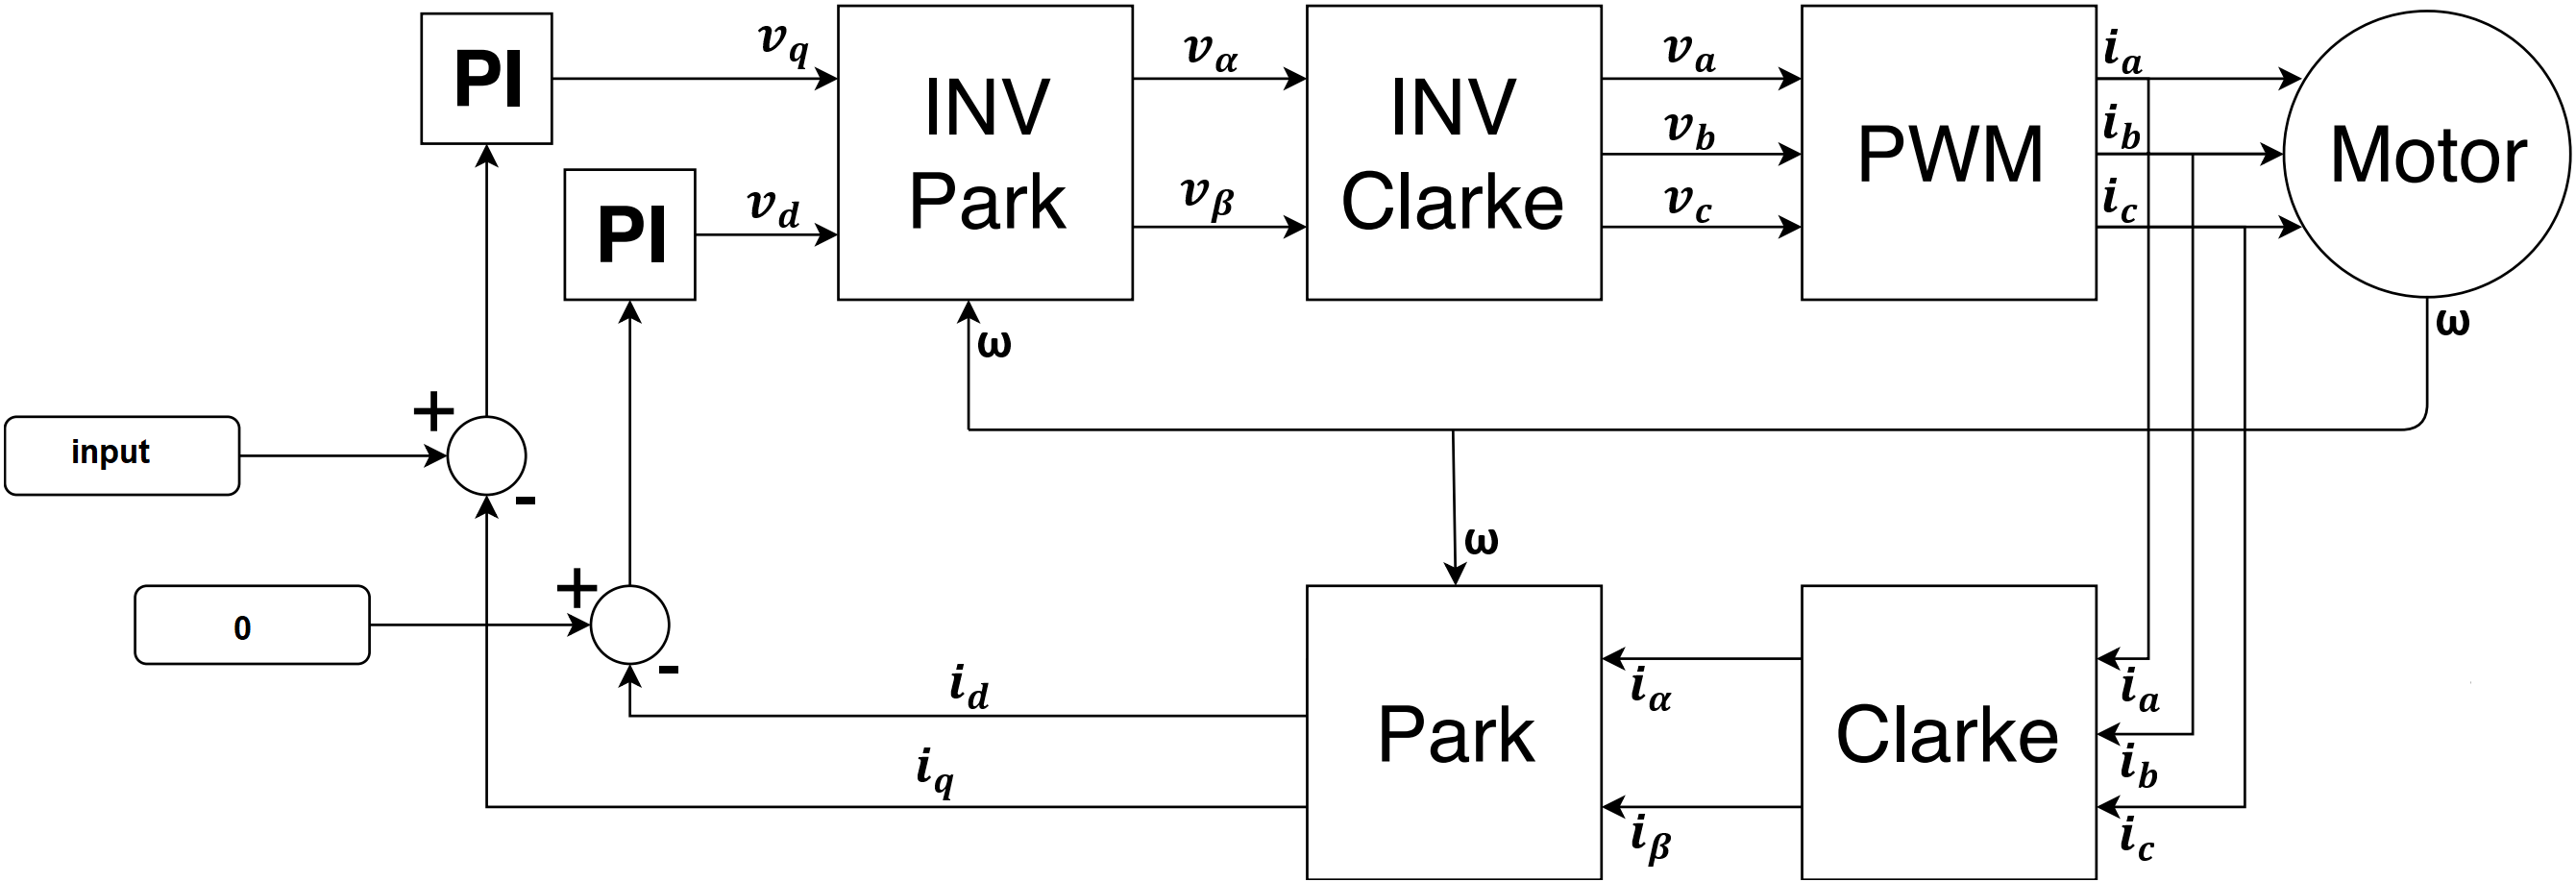
\includegraphics[scale=0.42]{pictures/control/udklip.PNG}
    \caption{Motor model used for the control as an overview.}
    \label{fig:Motor_model}
\end{figure} 

On the right the motor can be seen. The phase current out of the inverter is transformed into a rotating frame of reference by first performing a Clarke Transformation and then a Park Transformation. Out comes two signals $i_d$ and $i_q$ which goes into two individual controllers. FOC usually use PI controllers because only a proportional and a integrator part is needed.
The motor torque is biggest when the electric field is perpendicular to the rotor position.

The $i_d$ signal should always be $0$ because it resembles electric field not perpendicular to the rotor. Therefore it is subtracted with $0$ which makes $i_d$ the error and the signal is out into the PI controller. 
The $i_q$ resembles the electric field perpendicular to the rotor which is what produces the torque. Therefore this signal is compared with the input which is the target torque that comes from the torque pedal. After the PI controllers the two control signals in the rotating frame of reference are transformed back out into three phases with an Inverse Park Transformation and an Inverse Clarke Transformation. The signals can then be used to control the inverter.



% The model consist of two inputs where one is always , two PI controllers, and inverse Park and Clarke transformations, a motor with the data from \ref{Motor_parameters_list} and negative feedback transformed back with normal Park, Clarke transformation.\\

% The general idea behind model is having the input, being the wanted speed of the motor as a current, in go karts case it would be the torque pedal. The $0$ input is $0$ because of field oriented control, more on that in next section. The signal is then being tuned with the negative feedback and the controllers. Having the signal transformed is an important step, since a 3-phase motors needs 3 signals. The PWM box adjust the actual speed of the motor. The feedback comes from the 3 phases and the speed, that all help minimize errors in the signal. \\

% \subsubsection{Field oriented control}
% A couple of common techniques are generally to control motors. The calculations are usually scalar based or vector based, each having their usages. In this project the technique used is FOC, which is vector based. \\

% \begin{figure} [H]
%     \centering
%     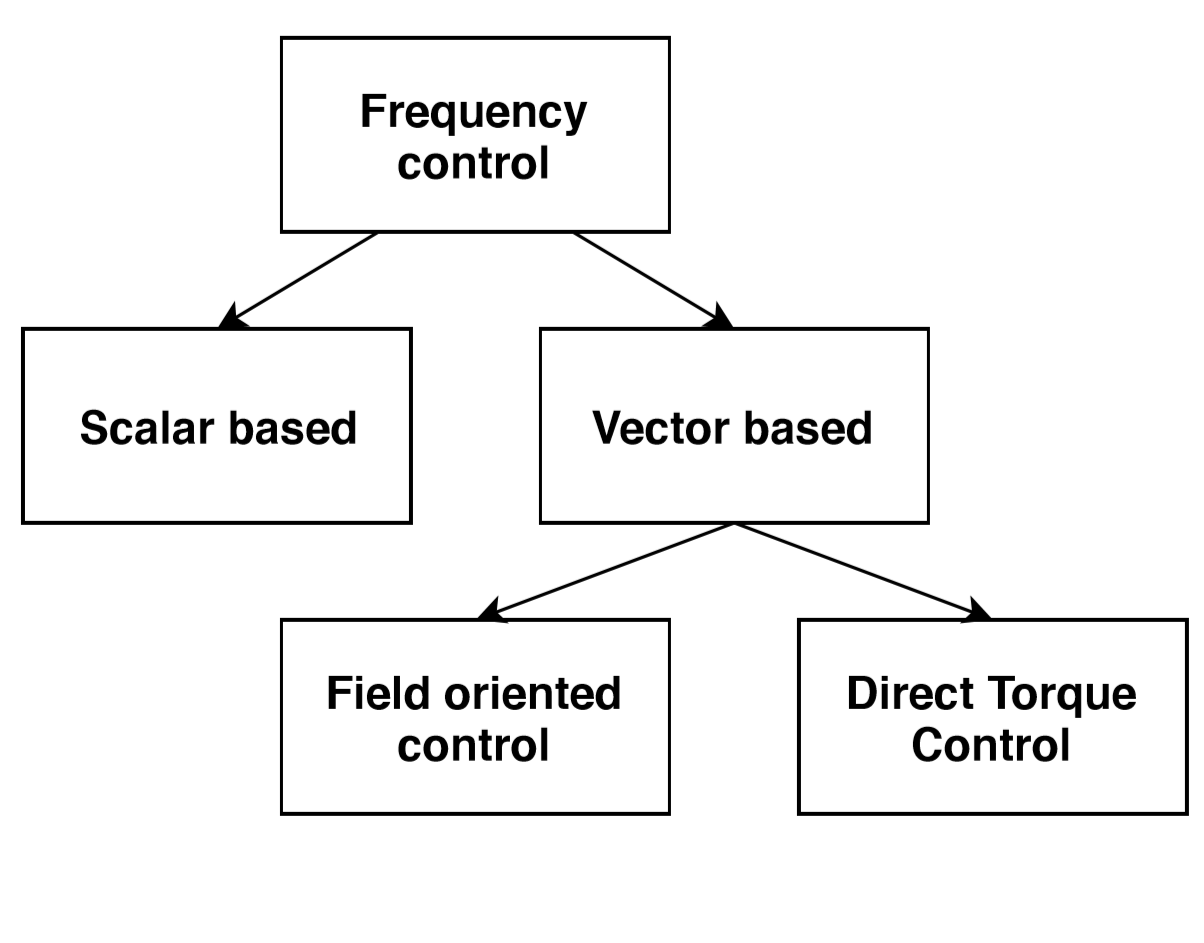
\includegraphics[scale=0.6]{pictures/control/udklip1.PNG}
%     \caption{An overview of where FOC is lays among frequency control}
%     \label{fig:my_label}
% \end{figure} 

% The reason for using FOC in this given project, is because it is relatively easy to use and implement. This method gives control over the current and voltages, and gives information about the orientation of the rotor, which gives smoother operation of the motor than normal PWM control. \\

% \begin{figure} [H]
%     \centering
%     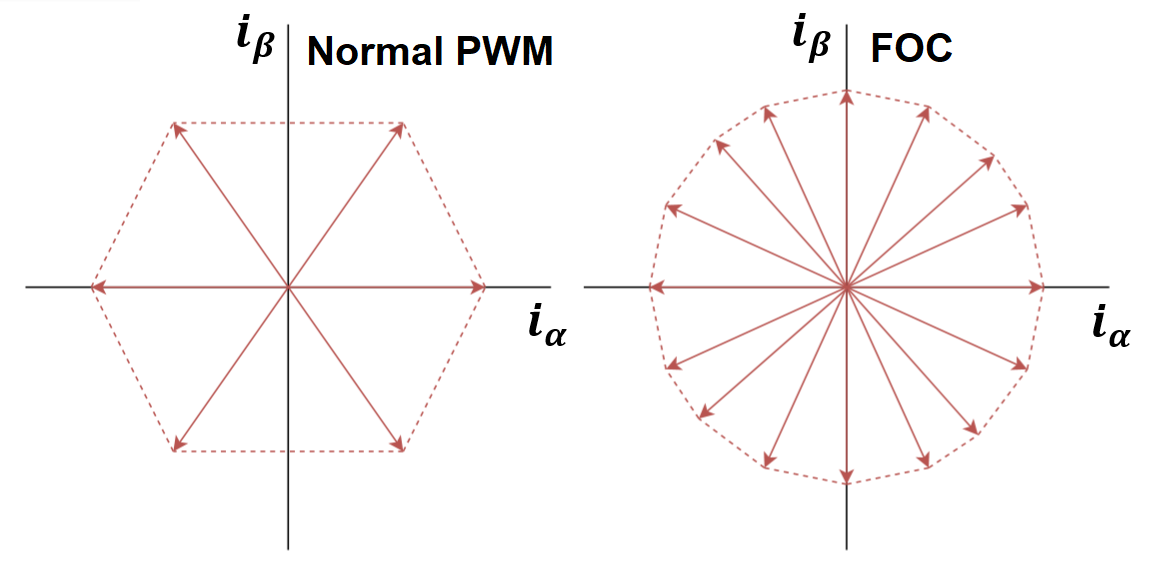
\includegraphics[scale=0.85]{pictures/control/Udklip2.PNG}
%     \caption{A visualization of how FOC gives higher control of the PWM signal, the red line representing more steps of where the magnetic field can be placed.}
%     \label{fig:my_label}
% \end{figure}

